\documentclass[]{book}
\usepackage{lmodern}
\usepackage{amssymb,amsmath}
\usepackage{ifxetex,ifluatex}
\usepackage{fixltx2e} % provides \textsubscript
\ifnum 0\ifxetex 1\fi\ifluatex 1\fi=0 % if pdftex
  \usepackage[T1]{fontenc}
  \usepackage[utf8]{inputenc}
\else % if luatex or xelatex
  \ifxetex
    \usepackage{mathspec}
  \else
    \usepackage{fontspec}
  \fi
  \defaultfontfeatures{Ligatures=TeX,Scale=MatchLowercase}
\fi
% use upquote if available, for straight quotes in verbatim environments
\IfFileExists{upquote.sty}{\usepackage{upquote}}{}
% use microtype if available
\IfFileExists{microtype.sty}{%
\usepackage{microtype}
\UseMicrotypeSet[protrusion]{basicmath} % disable protrusion for tt fonts
}{}
\usepackage[margin=1in]{geometry}
\usepackage{hyperref}
\hypersetup{unicode=true,
            pdftitle={Assessing the aging infrastructure through data-mining of the National Bridge Inventory: an exploratory analysis},
            pdfauthor={Alejandro Belenguer},
            pdfborder={0 0 0},
            breaklinks=true}
\urlstyle{same}  % don't use monospace font for urls
\usepackage{natbib}
\bibliographystyle{apalike}
\usepackage{longtable,booktabs}
\usepackage{graphicx,grffile}
\makeatletter
\def\maxwidth{\ifdim\Gin@nat@width>\linewidth\linewidth\else\Gin@nat@width\fi}
\def\maxheight{\ifdim\Gin@nat@height>\textheight\textheight\else\Gin@nat@height\fi}
\makeatother
% Scale images if necessary, so that they will not overflow the page
% margins by default, and it is still possible to overwrite the defaults
% using explicit options in \includegraphics[width, height, ...]{}
\setkeys{Gin}{width=\maxwidth,height=\maxheight,keepaspectratio}
\IfFileExists{parskip.sty}{%
\usepackage{parskip}
}{% else
\setlength{\parindent}{0pt}
\setlength{\parskip}{6pt plus 2pt minus 1pt}
}
\setlength{\emergencystretch}{3em}  % prevent overfull lines
\providecommand{\tightlist}{%
  \setlength{\itemsep}{0pt}\setlength{\parskip}{0pt}}
\setcounter{secnumdepth}{5}
% Redefines (sub)paragraphs to behave more like sections
\ifx\paragraph\undefined\else
\let\oldparagraph\paragraph
\renewcommand{\paragraph}[1]{\oldparagraph{#1}\mbox{}}
\fi
\ifx\subparagraph\undefined\else
\let\oldsubparagraph\subparagraph
\renewcommand{\subparagraph}[1]{\oldsubparagraph{#1}\mbox{}}
\fi

%%% Use protect on footnotes to avoid problems with footnotes in titles
\let\rmarkdownfootnote\footnote%
\def\footnote{\protect\rmarkdownfootnote}

%%% Change title format to be more compact
\usepackage{titling}

% Create subtitle command for use in maketitle
\newcommand{\subtitle}[1]{
  \posttitle{
    \begin{center}\large#1\end{center}
    }
}

\setlength{\droptitle}{-2em}

  \title{Assessing the aging infrastructure through data-mining of the National
Bridge Inventory: an exploratory analysis}
    \pretitle{\vspace{\droptitle}\centering\huge}
  \posttitle{\par}
    \author{Alejandro Belenguer}
    \preauthor{\centering\large\emph}
  \postauthor{\par}
      \predate{\centering\large\emph}
  \postdate{\par}
    \date{2018-12-22}

\usepackage{booktabs}

\usepackage{amsthm}
\newtheorem{theorem}{Theorem}[chapter]
\newtheorem{lemma}{Lemma}[chapter]
\theoremstyle{definition}
\newtheorem{definition}{Definition}[chapter]
\newtheorem{corollary}{Corollary}[chapter]
\newtheorem{proposition}{Proposition}[chapter]
\theoremstyle{definition}
\newtheorem{example}{Example}[chapter]
\theoremstyle{definition}
\newtheorem{exercise}{Exercise}[chapter]
\theoremstyle{remark}
\newtheorem*{remark}{Remark}
\newtheorem*{solution}{Solution}
\begin{document}
\maketitle

{
\setcounter{tocdepth}{1}
\tableofcontents
}
\chapter{Introduction}\label{intro}

The aging trend of the U.S. bridge inventory has been arisen by the ASCE
in the recent years \citep{asce2017InfrastructureReport2017}. An
increasing population of older bridges creates a challenging scenario
for the future bridge maintenance strategy. However, the observed
reduction of the structurally defficient bridges is a first step
forward.

\begin{figure}

{\centering 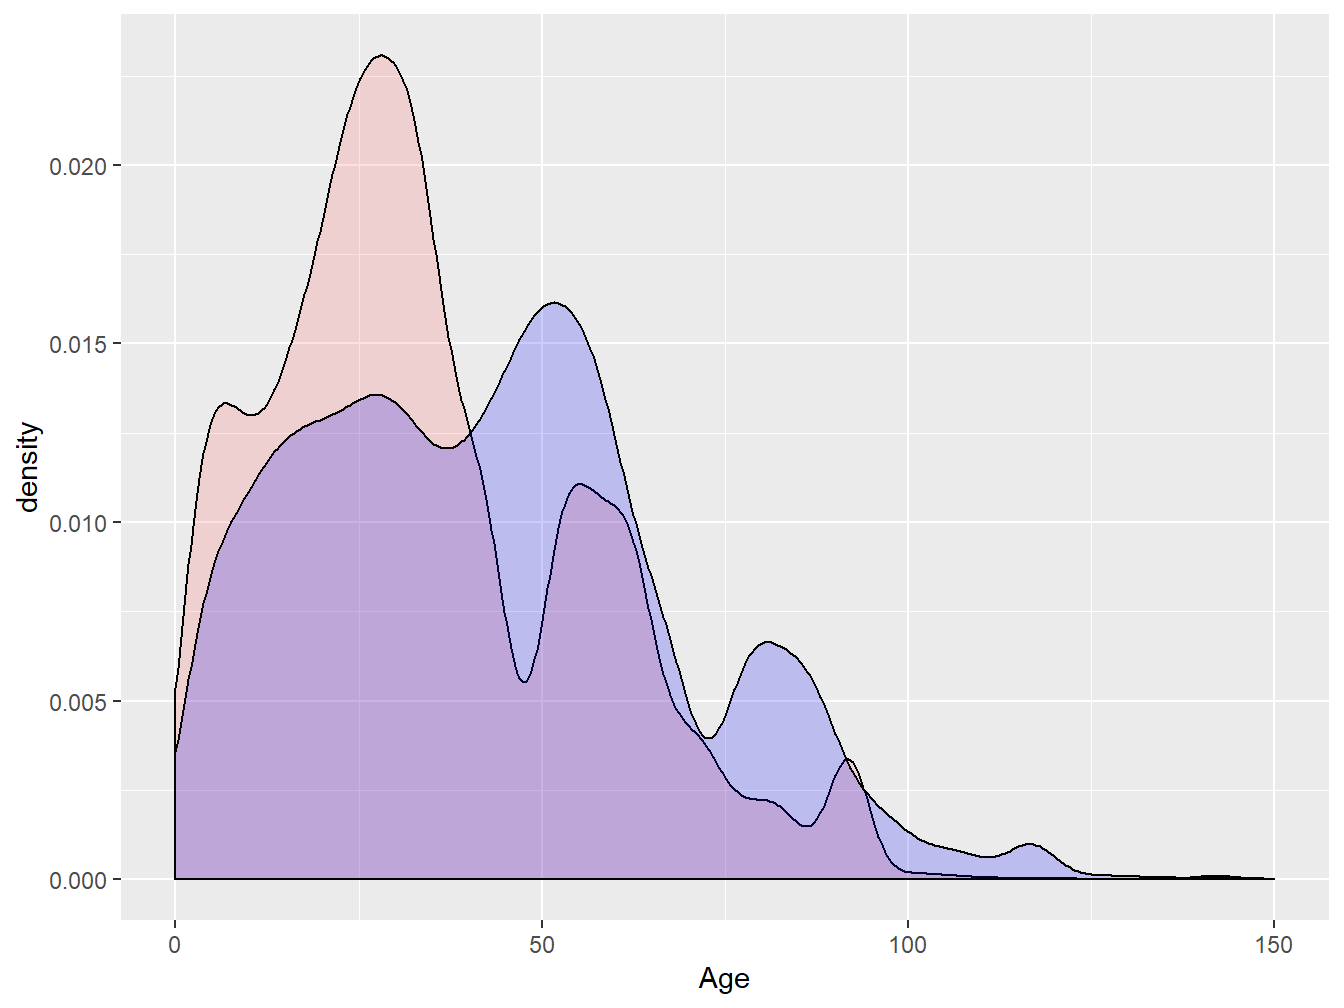
\includegraphics[width=0.8\linewidth]{CVEN6833-Project_files/figure-latex/bridge-age-1} 

}

\caption{Age distribution of US bridges (1992 vs. 2017)}\label{fig:bridge-age}
\end{figure}

Figure \ref{fig:bridge-age} shows the formentioned aging effect. The
data has been downloaded from the publicly accessible National Bridge
Inventory (NBI) of the U.S. Federal Highway Administration. The
horizontal shift between peak densities represent the time lag (26
years), while the vertical shift shows a decrease in the total
population density.

Stablishing the right criteria to sustain bridge condition on safe
levels is a key factor in a problem of limited resource allocation.
Thus, the study of the relation between bridge characteristics and
bridge performance can uncover better bridge maintenance policies.

\chapter{Previous techniques and
methods}\label{previous-techniques-and-methods}

The NBI has been previously exploited to predict bridge ratings,
i.e.~structural condition, from different elements such as deck,
superstructure, substructure, or culvert. The vast amount of data
available, totalling more than 600,000 bridges, has been tackled by
subsetting the inventory into smaller samples using different criteria.
\citet{contreras-nietoDevelopmentLinearModels2014} used the steel and
prestressed concrete bridges in Oklahoma, while
\citet{saeedPerformanceEvaluationLife2017} worked on the Indiana
database.

Related studies have been carried out using neural networks, Markov
models, and regression trees
\citep{veshoskyComparativeAnalysisBridge1994} to the bridge
superstructure condition.
\citet{bektasbasakaldemirUsingClassificationTrees2013} applied
classification and regression trees to predict bridge ratings and later
on used recursive partitioning
\citet{bektasUseRecursivePartitioning2017}.

According to \citet{contreras-nietoCharacterizationSteelBridge2018}, in
the majority of the previous studies the model validation was not
performed and the results showed a low adjusted \(R^2\) value (around
0.4). This problem resulted in the unability of the models to predict
structurally deficient ratings, as they only represent a small fraction
(6\% - 9\%) of the inventory.

\chapter{Research problem}\label{research-problem}

This work tries to provide a better insight into the topic by using
novel data mining techniques. In particular, three non-supervised
learning techniques will be used to generate ``statistically similar''
subsets of data.

The first one used is the clustering of extremes (partition around
medioids) technique \citep{brackenSpatialVariabilitySeasonal2015}. As a
second approach, a classical Principal Component Analysis is carried
out. Finally, Self-Organizing Maps will be used to compare with previous
results.

With the results from the non-supervised approach, a multinomial
regression will be used to predict the strucural condition of the
bridges, and compare those with regression models without previous
clustering.

\section{Description of the data}\label{description-of-the-data}

The NBI database accounts for more than 136 parameters of the bridge
inventory gathered at each bridge inspection. More information about the
methodology can be consulted in the Recording and coding guide for the
structure inventory and appraisal of the nation's bridges
\citet{wesemanRecordingCodingGuide1995}.

The forementioned previous work found a fraction of those variables to
be statistically significant when using regression models to predict
bridge condition. Working from those, the author has selected the same
to guarantee enough breadth of scope in the analysis.

\begin{table}[t]

\caption{\label{tab:tab-01}Selected variables}
\centering
\begin{tabular}{llll}
\toprule
Variable & Code number & Numeric type & Temporal type\\
\midrule
Structure number & 008 & Character & Stationary\\
Latitude & 016 & Numeric & Stationary\\
Longitude & 017 & Numeric & Stationary\\
Year built & 027 & Numeric & Stationary\\
Average Daily Traffic & 029 & Numeric & Time series\\
\addlinespace
Design load & 031 & Binary & Stationary\\
Service under bridge & 042B & Categorical & Stationary\\
Structure kind & 043A & Categorical & Stationary\\
Structure type & 043B & Categorical & Stationary\\
Length of maximum span & 048 & Numeric & Stationary\\
\addlinespace
Structure length & 049 & Numeric & Stationary\\
Bridge roadway width & 051 & Numeric & Stationary\\
Deck Condition & 058 & Categorical & Time series\\
Superstructure condition & 059 & Categorical & Time series\\
Substructure condition & 060 & Categorical & Time series\\
\addlinespace
Culvert condition & 062 & Categorical & Time series\\
Year reconstructed & 106 & Binary & Time series\\
Percentage of Truck in ADT & 109 & Numeric & Time series\\
\bottomrule
\end{tabular}
\end{table}

The table \ref{tab:tab-01} summarizes the variables names and numeric
type adopted departing from \citet{wesemanRecordingCodingGuide1995}. In
order to simplify the anlysis, some variables have been transformed,
according to the following description:

\begin{enumerate}
\def\labelenumi{\arabic{enumi}.}
\item
  Latitude, Longitude: considered full numeric precision available
  (hundredths of a second).
\item
  Year built: used to calculate bridge age.
\item
  ADT: considered full precision. However, the variable considered has
  been the Truck Average Daily Traffic, as it is the one considered
  significant \citep{saeedPerformanceEvaluationLife2017}. The TADT is
  obtained multiplicating the ADT by the percentage of trucks in ADT
  (code 109).
\item
  Design load. Transformed to binary. 1 if code is known, 0 if not.
\item
  Structure kind and type: the original data considers different
  building materials for the first case, and different bearing
  mechanisms for the latter. The bridge selection process lead to
  consider only three kinds of superstructure material: steel,
  reinforced concrete, and prestressed concrete. Similarly, the most
  frequent structural type was girder / multibeam bridge. Thus, only
  this category was retained.
\item
  Length of maximum span: only bridges between 15 and 50 m. of maximum
  span length have been considered with the objective of comparing
  similar structures. Within the range, full numeric values are used.
  Figures \ref{fig:max-span} and \ref{fig:max-span-cut} show the process
  followed.
\end{enumerate}

\begin{figure}

{\centering 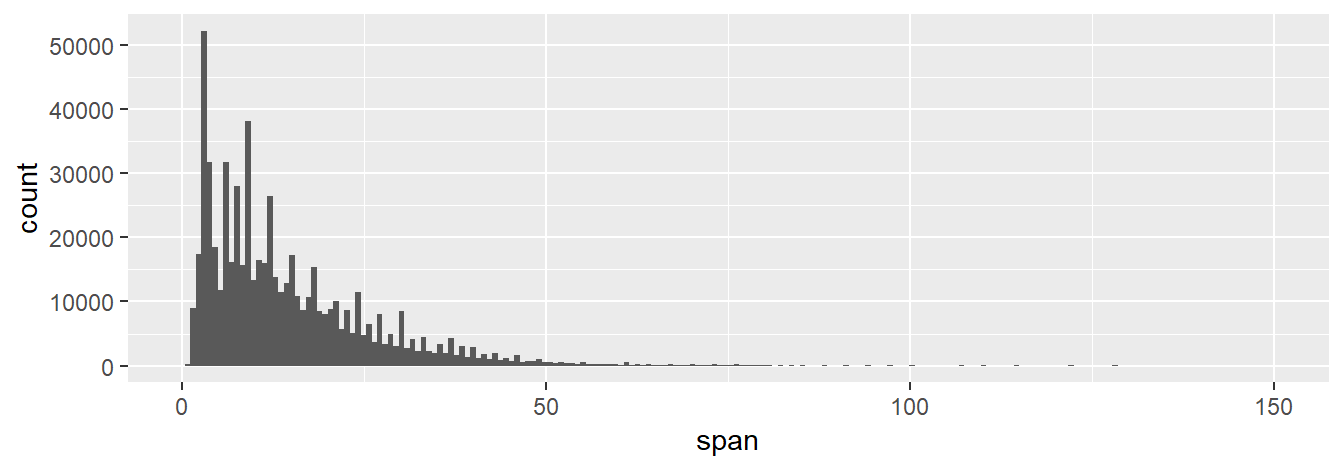
\includegraphics[width=0.8\linewidth]{CVEN6833-Project_files/figure-latex/max-span-1} 

}

\caption{Max. span length distribution of selected bridges}\label{fig:max-span}
\end{figure}\begin{figure}

{\centering 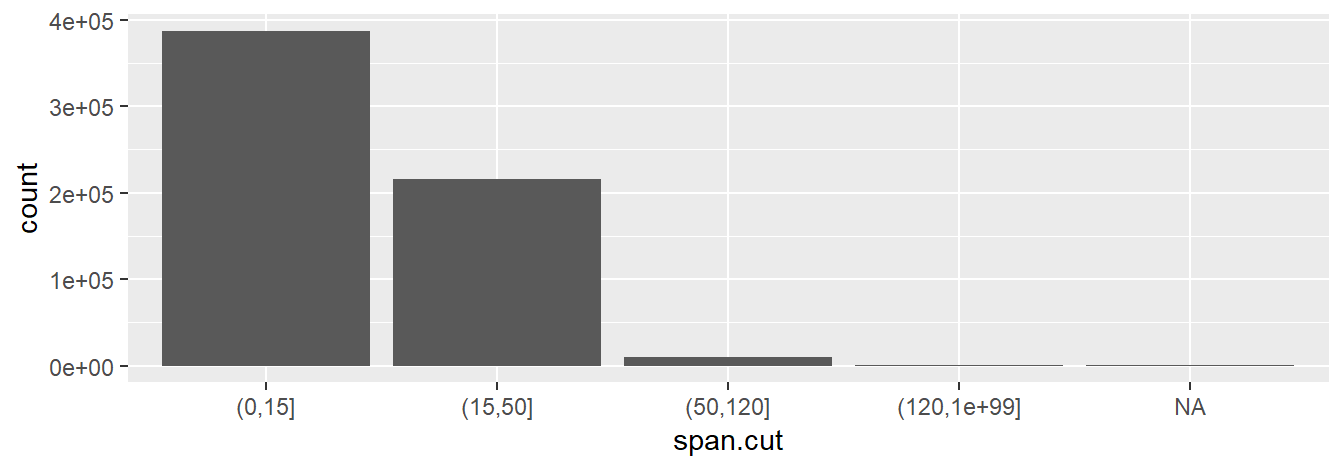
\includegraphics[width=0.8\linewidth]{CVEN6833-Project_files/figure-latex/max-span-cut-1} 

}

\caption{Max. span length bins used to select bridges for the analysis}\label{fig:max-span-cut}
\end{figure}

\begin{enumerate}
\def\labelenumi{\arabic{enumi}.}
\setcounter{enumi}{6}
\item
  Structure length: The wide range of lengths was transformed into four
  bins: from 15 to 50 m., from 50 to 100 m., from 100 to 200 m., and
  longer. The median length values were used to replace previous values
  (25, 75, 150, and 500 m., respectively).
\item
  Bridge total width: full numeric precision considered.
\item
  Deck, superstructure, substructure, and culvert condition: Original
  data adopted a 0 to 9 scale to classify the specific bridge condition.
  However, a new variable considering the structural deficiency has been
  used to reflect the definition given by the Federal Highway
  Administration. The term is defined as the classification given to a
  bridge which has any component (Item 58, 59, 60, or 62) in Poor or
  worse condition (code of 4 or less).
\item
  Year reconstructed: A fraction of the bridges has had major
  interventions that exceed the regular maintenance practice. A binary
  variable indicating if a reconstruction has existed at a given year
  has been used to increase regression accuracy.
\end{enumerate}

\section{Hypothesis and diagnostics}\label{hypothesis-and-diagnostics}

The selected covariates were used to generate a subset of the entire
dataset. The criteria followed to reduce the number of case studies was
directly related to quality control and easiness of manipulation.

First, only bridges with the same name in 1992 and 2017 were retained.
All bridges been replaced or renamed were consequently excluded.
Additionally, only bridges with known location were included. Note that
older bridges are a consequence of choosing this criteria, as shown in
figure \ref{fig:age-select}.

\begin{figure}

{\centering 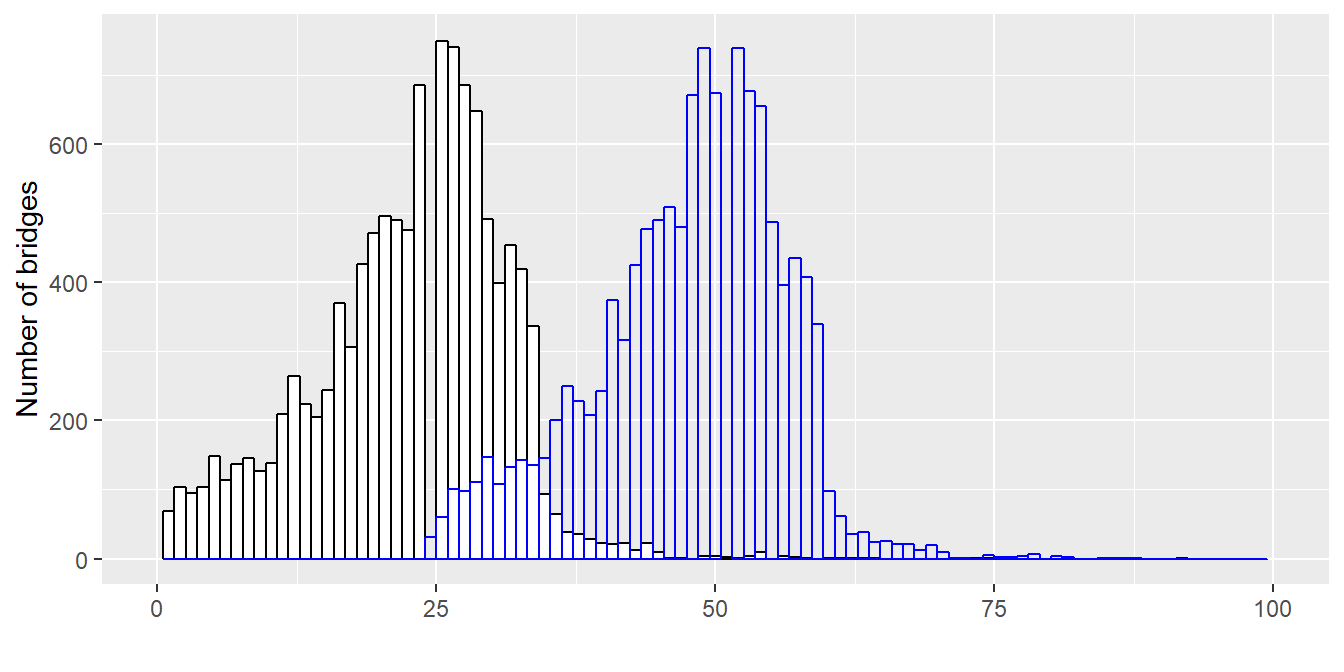
\includegraphics[width=0.8\linewidth]{CVEN6833-Project_files/figure-latex/age-select-1} 

}

\caption{Age of selected bridges (1992 vs. 2017)}\label{fig:age-select}
\end{figure}

Second, the condition rating of the selected bridges had to be known.
The values were in a few cases omitted for certain intermediate years.
In this cases the previous known value was used to generate continuous
data. Figures \ref{fig:cond-mean} and \ref{fig:cond-min} depict the how
fewer structurally deficient bridges and greater close-to-deficiency
bridges phenomena occur simultaneously.

\begin{figure}

{\centering 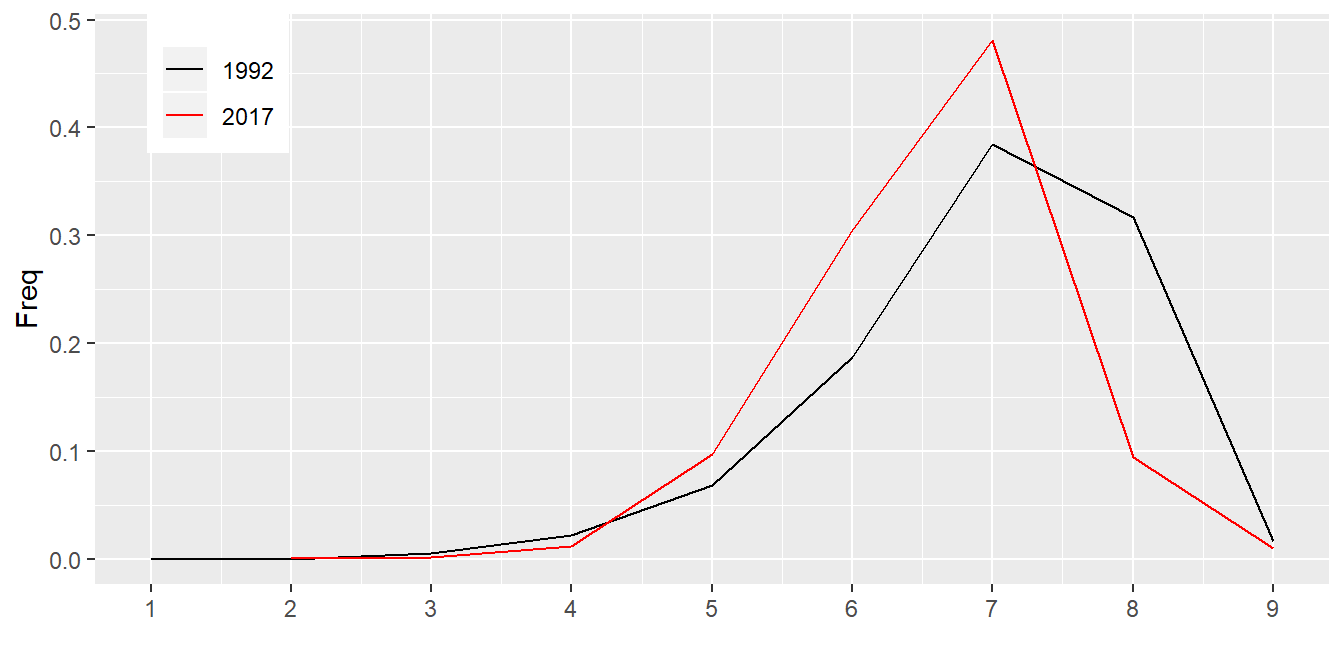
\includegraphics[width=0.8\linewidth]{CVEN6833-Project_files/figure-latex/cond-mean-1} 

}

\caption{Mean condition of selected bridges (1992 vs. 2017)}\label{fig:cond-mean}
\end{figure}\begin{figure}

{\centering 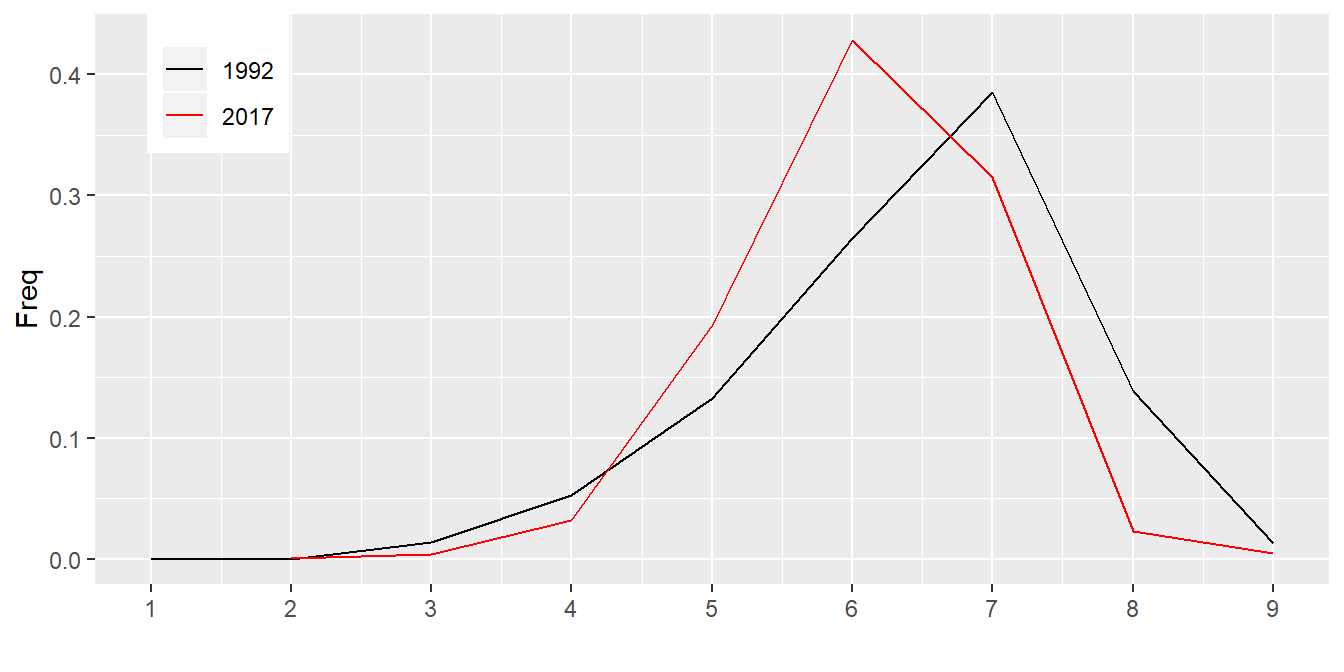
\includegraphics[width=0.8\linewidth]{CVEN6833-Project_files/figure-latex/cond-min-1} 

}

\caption{Minimum condition of selected bridges (1992 vs. 2017)}\label{fig:cond-min}
\end{figure}

Third, the maximum span length, structure kind, and structure type
matched the criteria described above. Only 15-50 max. span,
steel/concrete/prestressed concrete, multibeam bridges were then
considered. Figures \ref{fig:maxspan-dist}, \ref{fig:span-dist}, and
\ref{fig:width-dist} show the property distribution on the selected
bridges.

\begin{figure}

{\centering 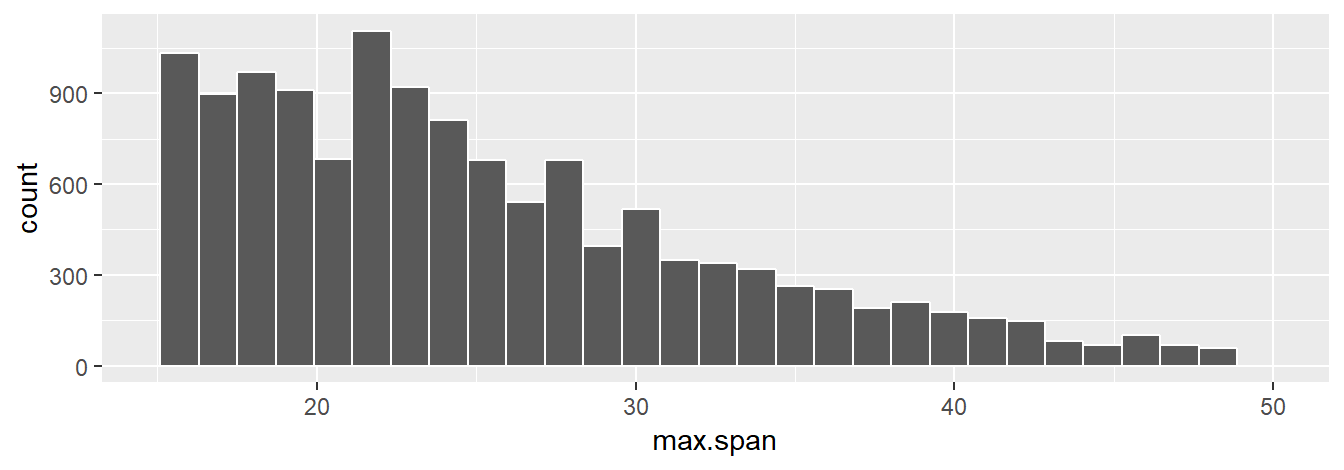
\includegraphics[width=0.8\linewidth]{CVEN6833-Project_files/figure-latex/maxspan-dist-1} 

}

\caption{Distribution of max. span on selected bridges}\label{fig:maxspan-dist}
\end{figure}\begin{figure}

{\centering 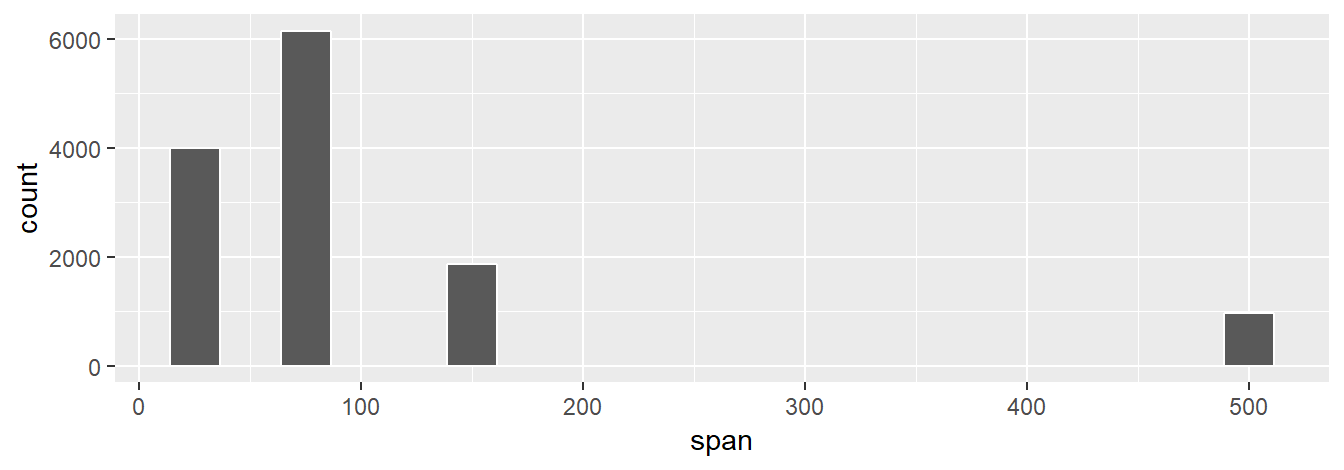
\includegraphics[width=0.8\linewidth]{CVEN6833-Project_files/figure-latex/span-dist-1} 

}

\caption{Distribution of total length on selected bridges}\label{fig:span-dist}
\end{figure}\begin{figure}

{\centering 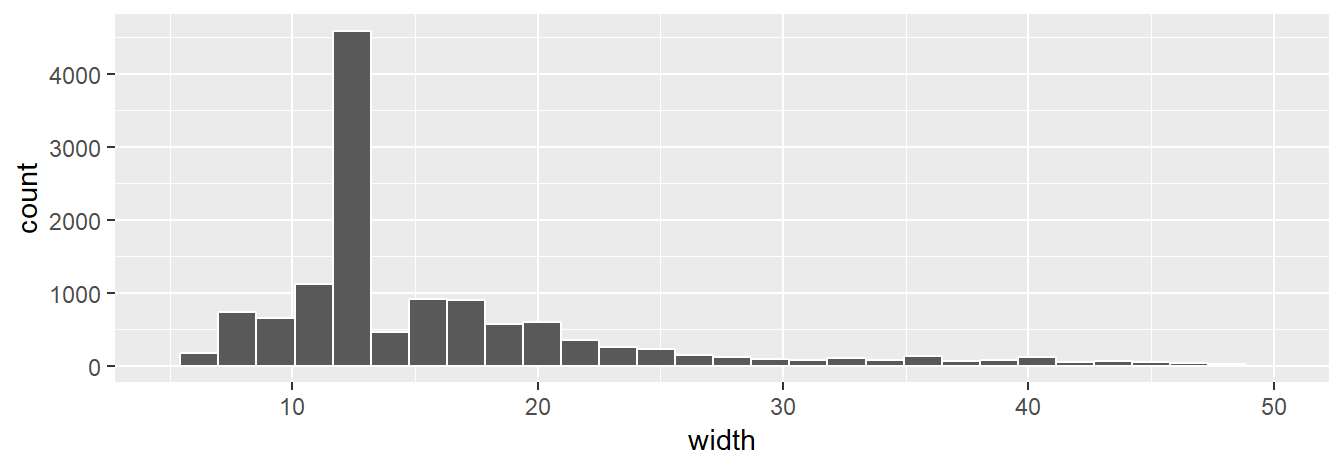
\includegraphics[width=0.8\linewidth]{CVEN6833-Project_files/figure-latex/width-dist-1} 

}

\caption{Distribution of bridge width on selected bridges}\label{fig:width-dist}
\end{figure}

Finally, only bridges in the continental US STRANHET corridors were
used. The STRAHNET corridor is formed by those highways considered
strategically important to the defense of the United States.

A total sample of 12,970 bridges scattered throughout the entire
continental US was used in the analysis, including 26 years of record.
Figure \ref{fig:age-span} maps them on the US territory.

\begin{figure}

{\centering 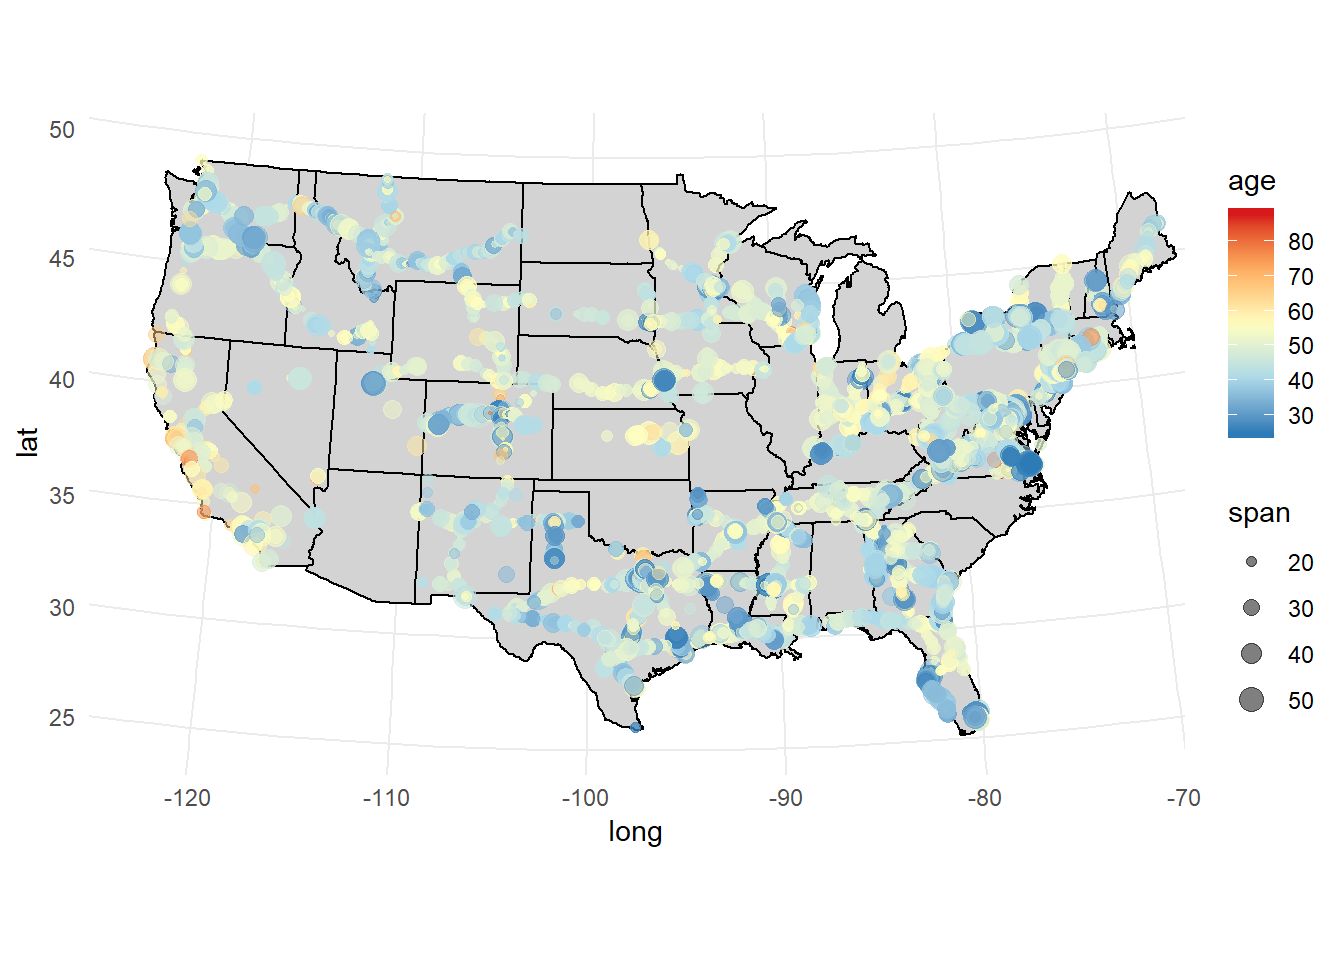
\includegraphics[width=1\linewidth]{CVEN6833-Project_files/figure-latex/age-span-1} 

}

\caption{Age and span spatial distribution of selected bridges (2017)}\label{fig:age-span}
\end{figure}

The resulting distribution of the structural condition for the time
series is, on average: * Structurally deficient (rating of 4 or under):
3.86 \% * At risk of being deficient (rating of 5): 15 \% *
Non-deficient: 81.13 \%

\chapter{Methodology and results}\label{methodology-and-results}

\section{Extreme Clustering}\label{extreme-clustering}

The first analysis consisted of a modification of a clustering technique
- partition around medoids - used in
\citet{brackenSpatialVariabilitySeasonal2015}.

3,000 case studies were randomly sampled from the selected data to
alleviate the simulation. The structural condition time series and the
lat, long position of the sample was the only variables provided. A
range from 2 to 20 clusters was analyzed. Figures \ref{fig:pam-2cluster}
and \ref{fig:pam-6cluster} show the optimal and third-best performance
according to the average silhouette method reproduced in figure
\ref{fig:pam-silh}.

\begin{figure}

{\centering 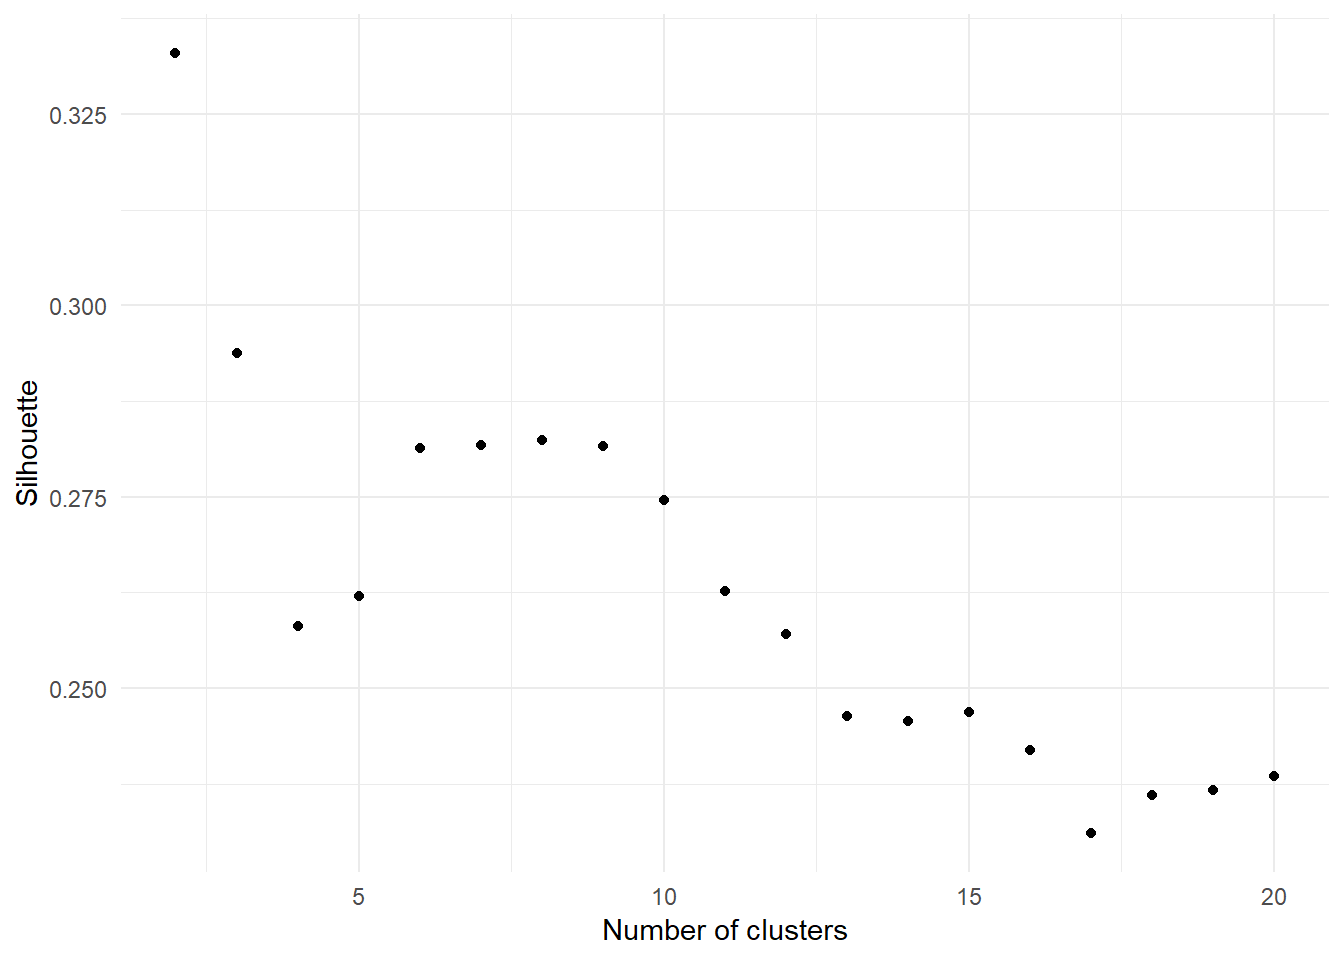
\includegraphics[width=0.8\linewidth]{CVEN6833-Project_files/figure-latex/pam-silh-1} 

}

\caption{Average silhouete profile for each number of clusters}\label{fig:pam-silh}
\end{figure}\begin{figure}

{\centering 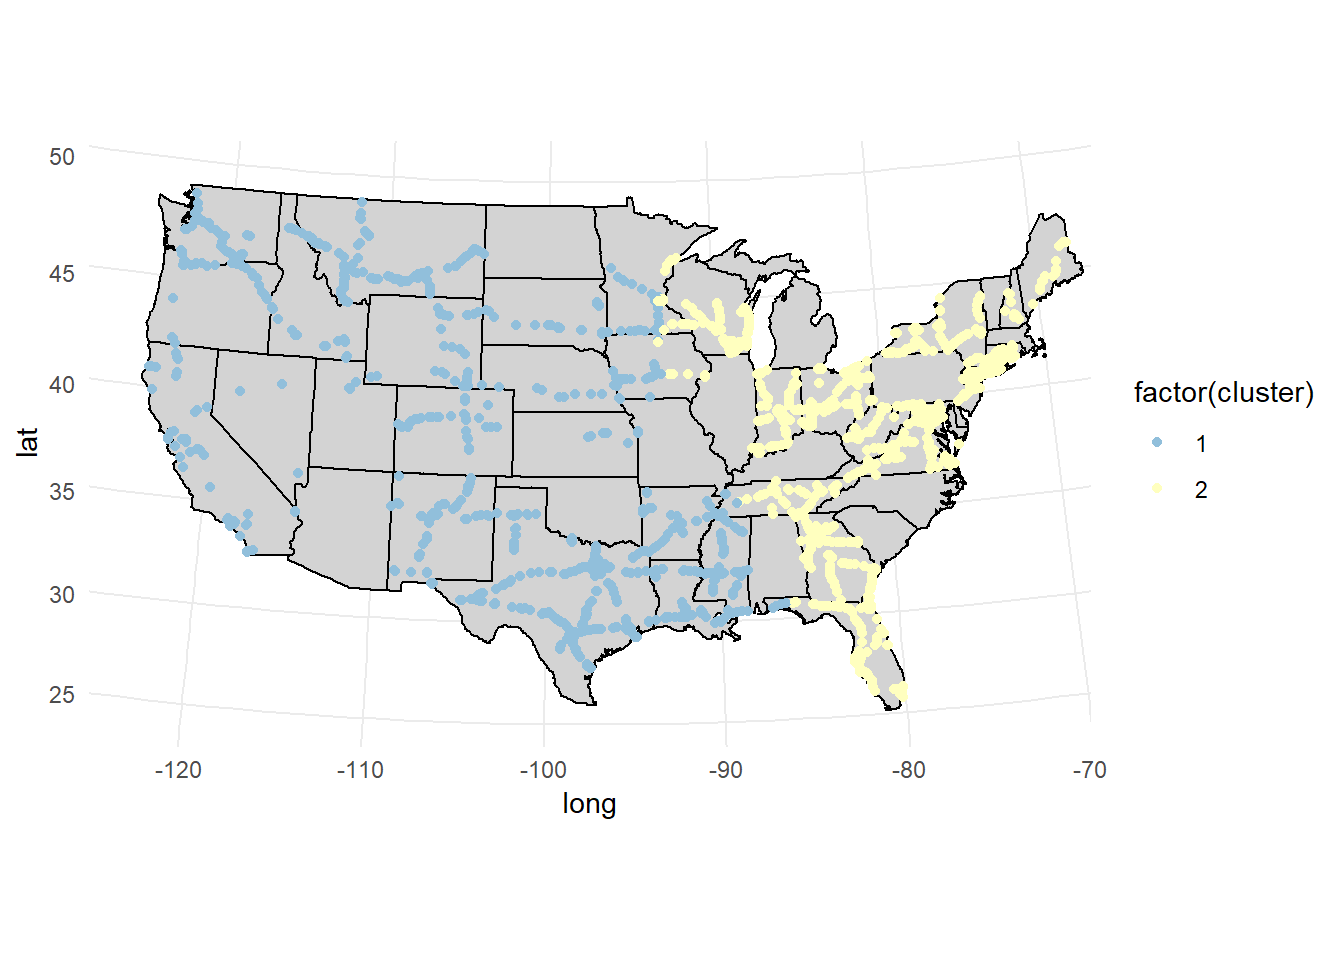
\includegraphics[width=0.8\linewidth]{CVEN6833-Project_files/figure-latex/pam-2cluster-1} 

}

\caption{Optimal PAM 2 - Clusters}\label{fig:pam-2cluster}
\end{figure}\begin{figure}

{\centering 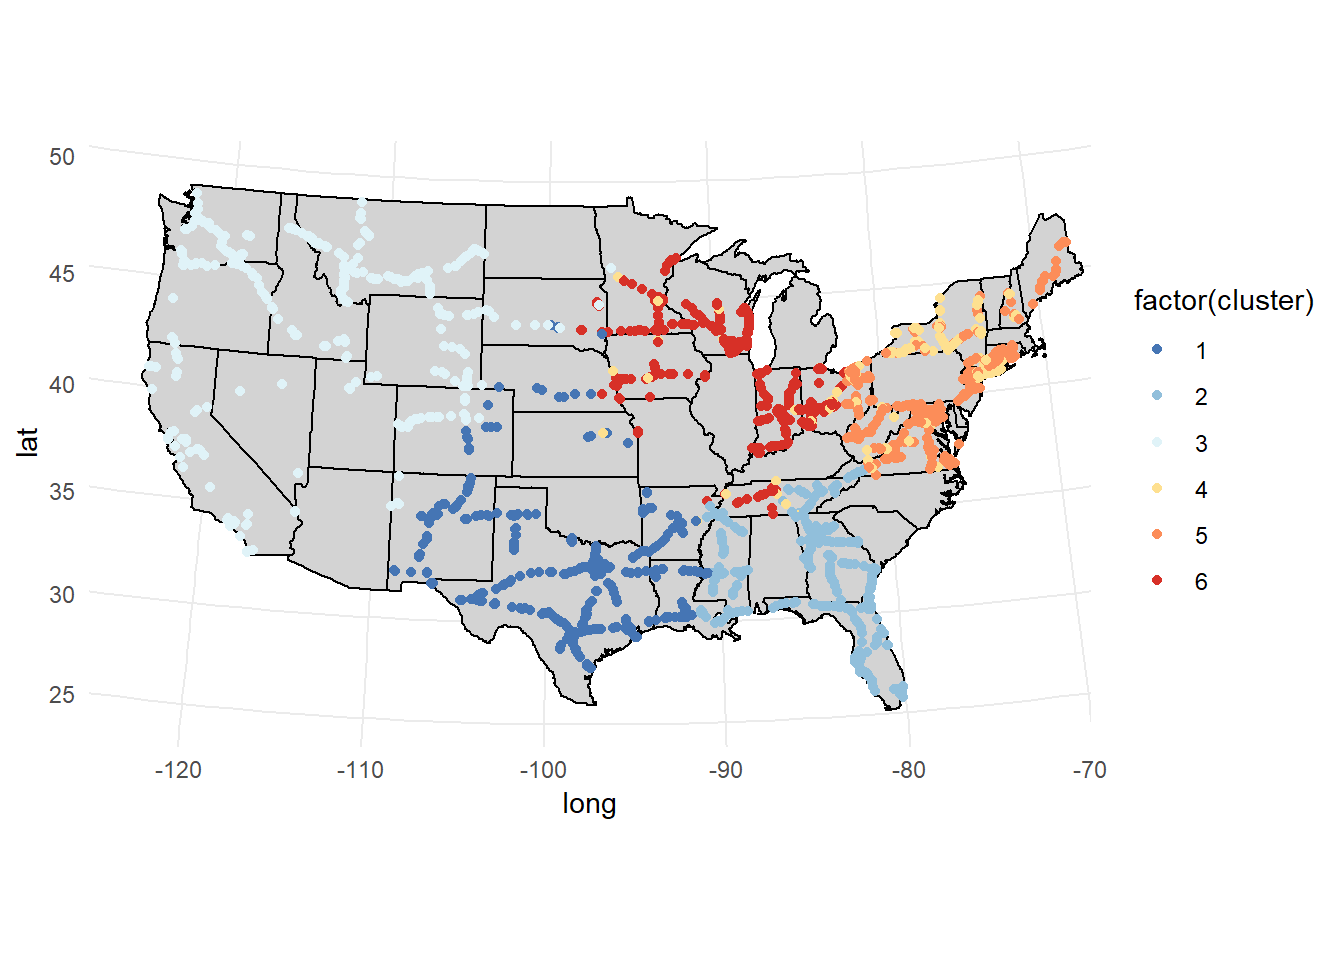
\includegraphics[width=0.8\linewidth]{CVEN6833-Project_files/figure-latex/pam-6cluster-1} 

}

\caption{Sub-optimal PAM 5 - Clusters}\label{fig:pam-6cluster}
\end{figure}

The similarity between the pattern showed by the 6-cluster simulation
and the North American Climate zones/types made us reflect about a
potential connection. That is why new variables associated with monthly
extreme temperatures and annual precipitation were added as covariates.

\begin{figure}
\centering
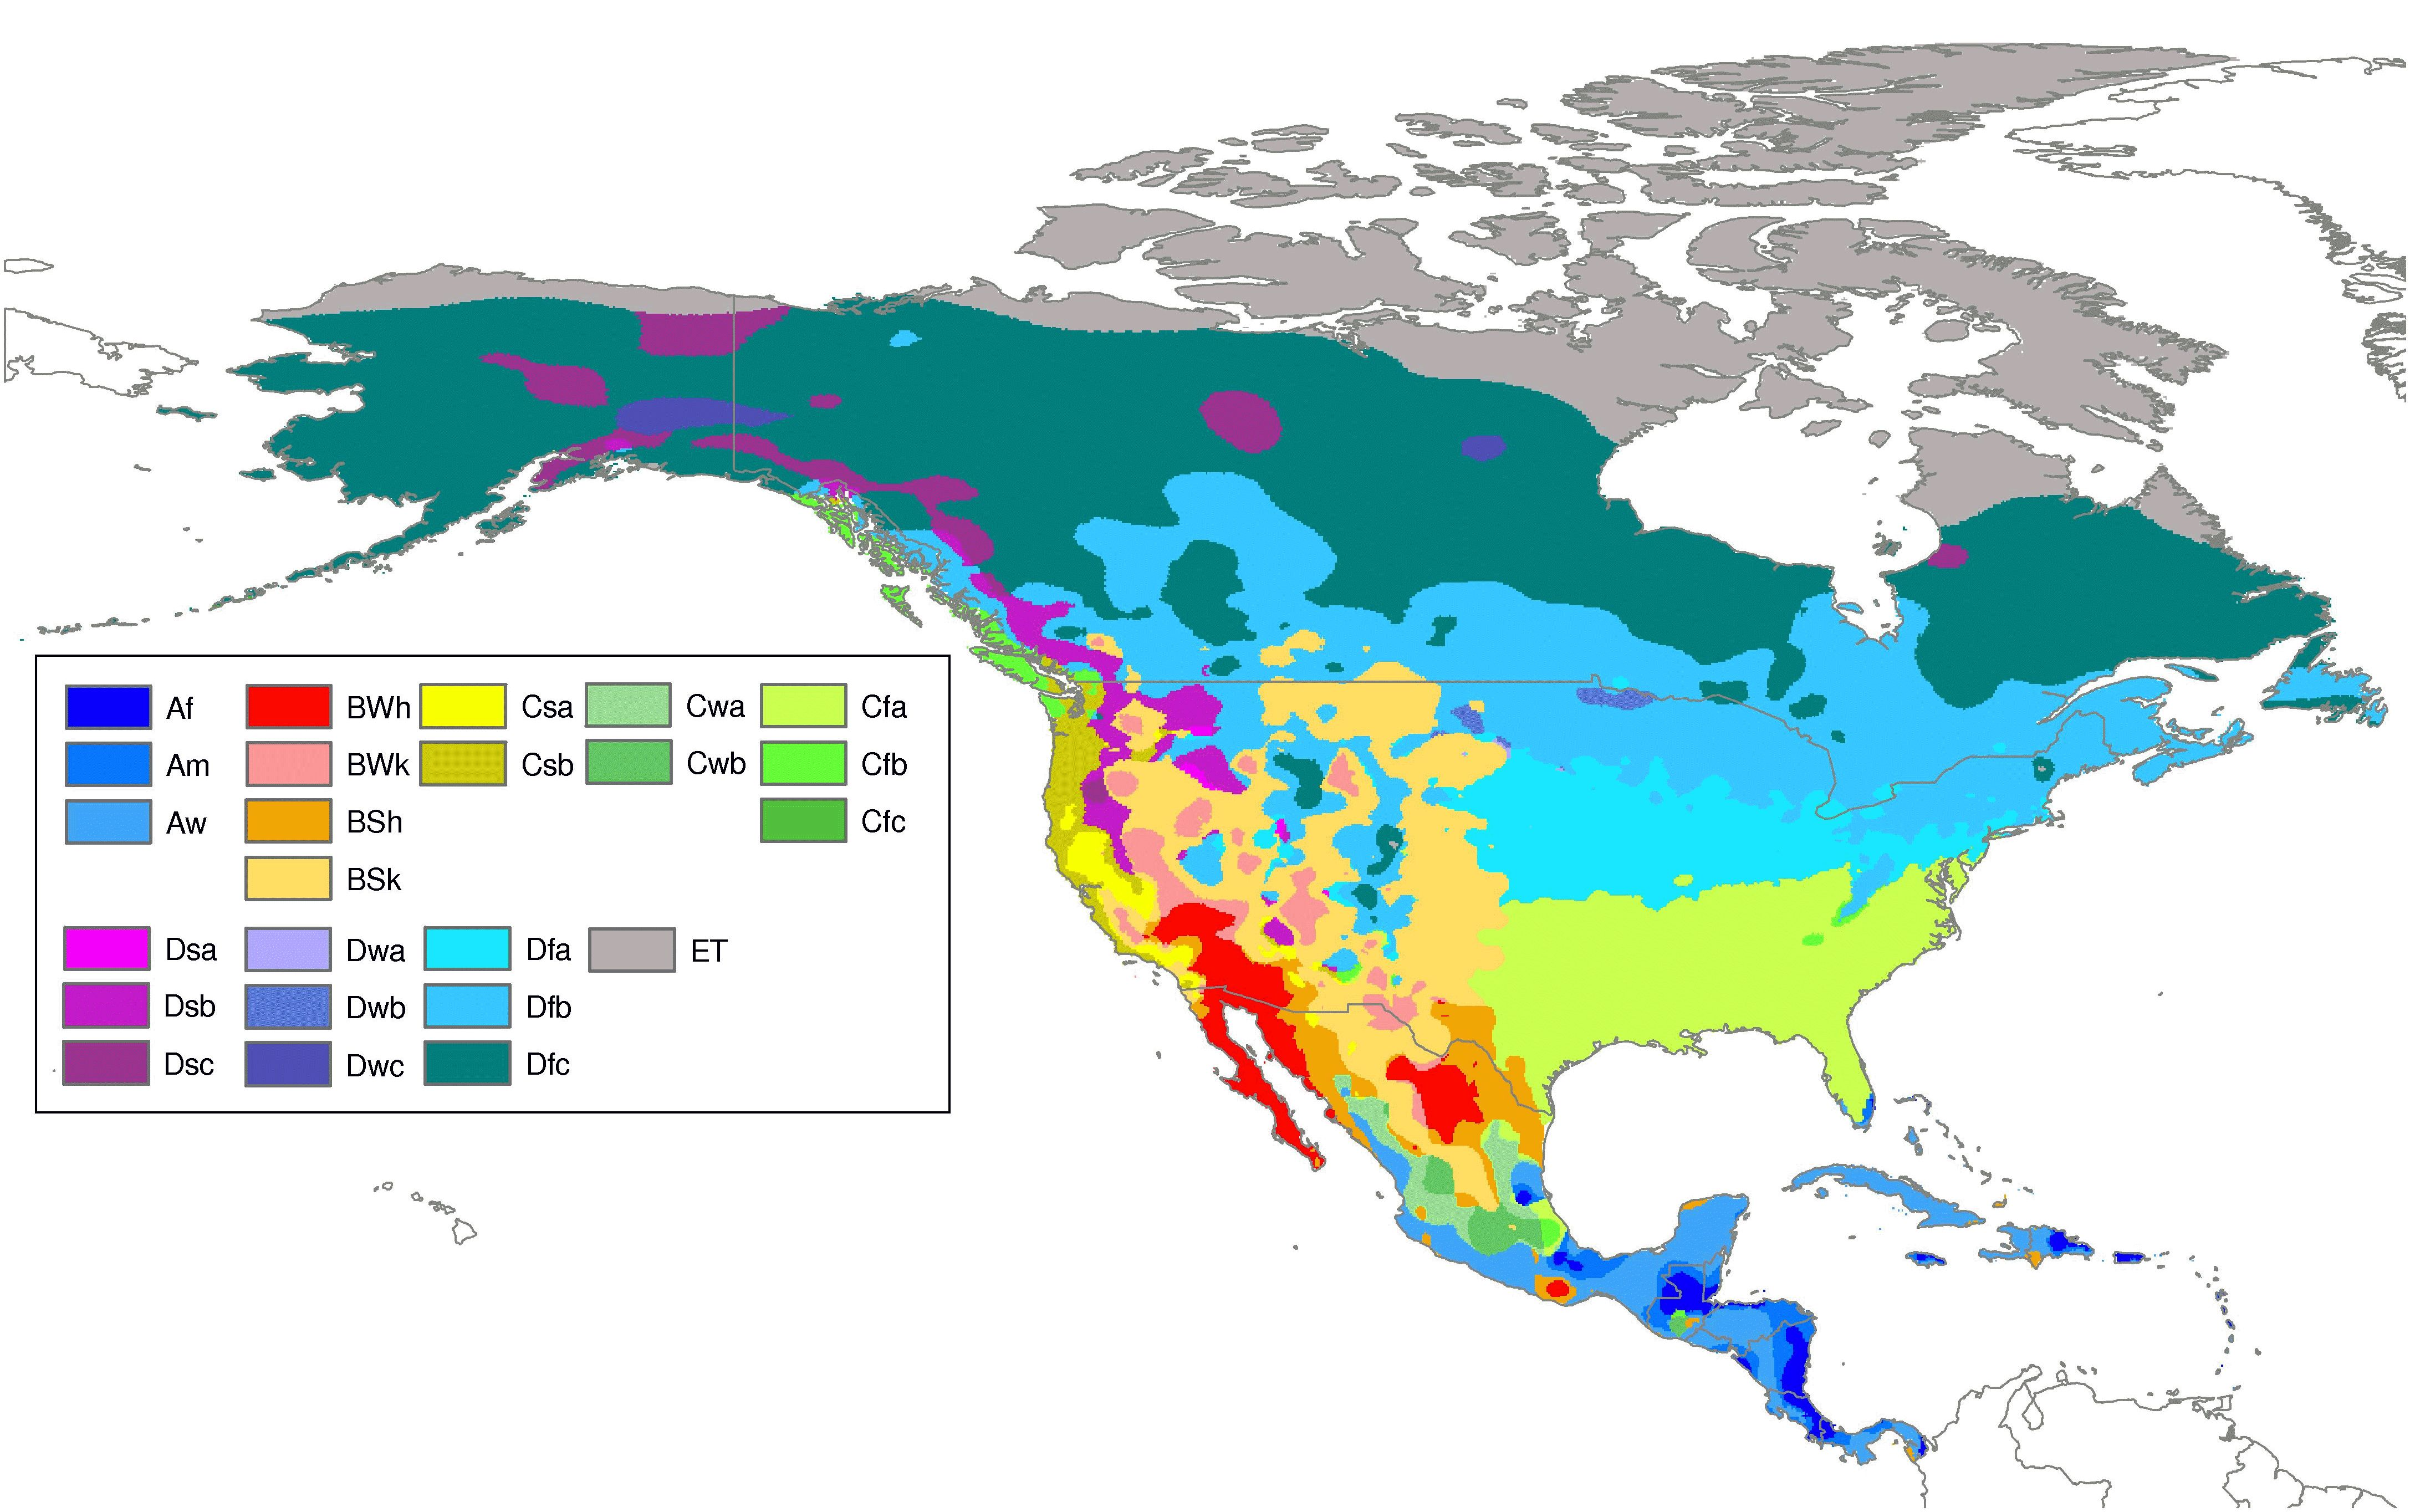
\includegraphics{North_America.jpg}
\caption{Climate types according to Koppen classification}
\end{figure}

\subsection{Adding climate variables to bridge
location}\label{adding-climate-variables-to-bridge-location}

Monthly climate-division data from the National Centers for
Environmental Information \citep{voseImprovedHistoricalTemperature2014}
was collected for the period 1991-2017. For each of the 344 datapoints
scatterd throughout the Continental US, the anual monthly maximum and
minimum temperature and annual precipitation was aggregated.

To translate this information into bridge-located data, a local
polynomial regression with a low alpha (0.05) and linear degree was used
for each climate variable. Fig

\begin{figure}

{\centering 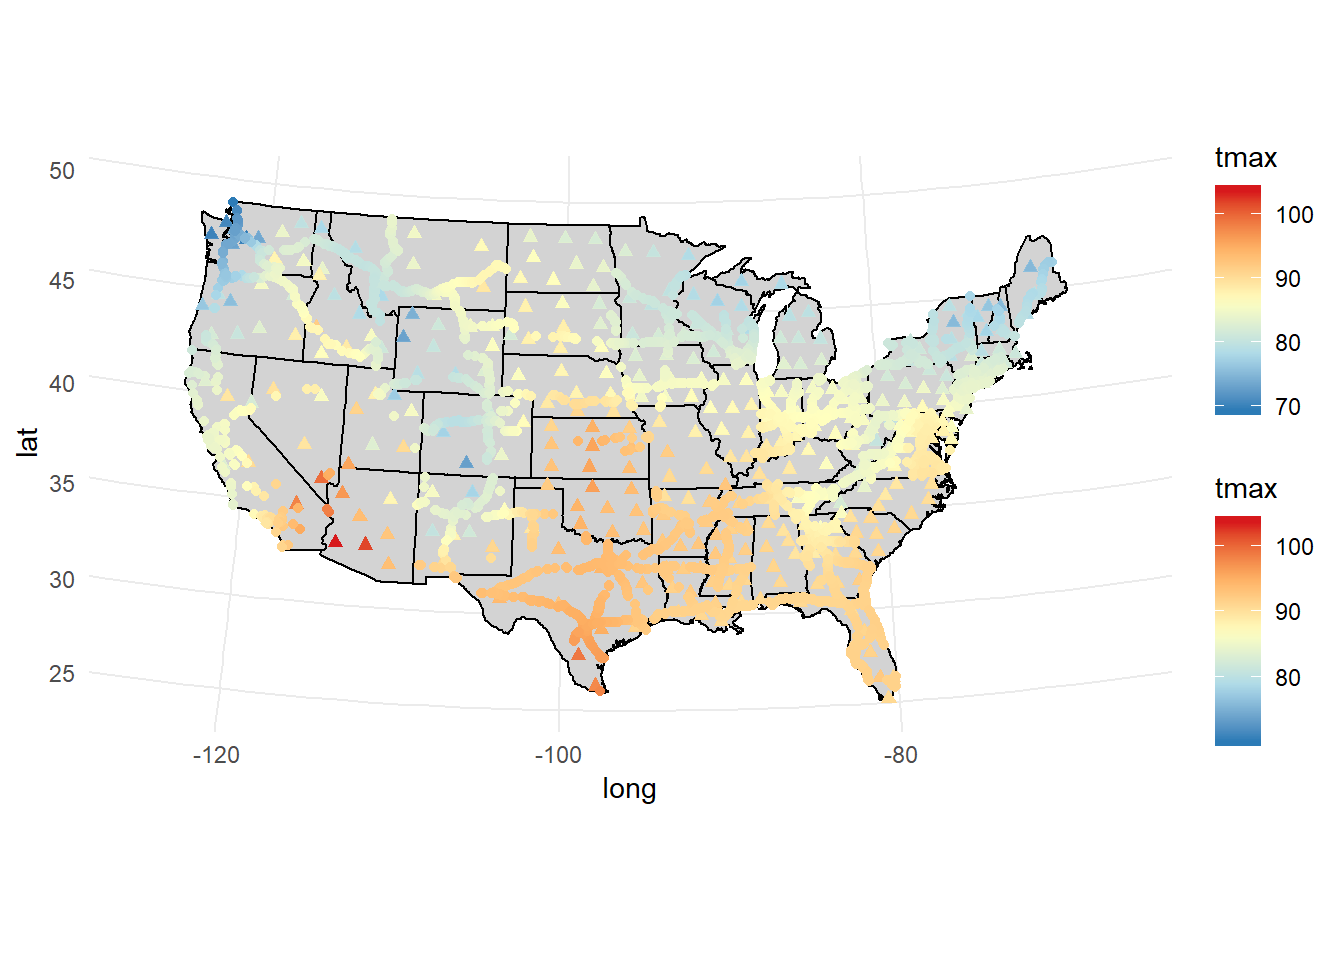
\includegraphics[width=0.8\linewidth]{CVEN6833-Project_files/figure-latex/clim-reg-1} 

}

\caption{1992 Annual maximum temperature - nClimDiv data and locfit regression}\label{fig:clim-reg}
\end{figure}

\section{Principal Component
Analysis}\label{principal-component-analysis}

A second analysis was carried out using PCA. In this case all variables
with exception of the deficiency condition of the bridge were considered
in the simulation. As a first approach, the climate variables were not
included (Fig. \ref{fig:lambdas}). Repeating the process with tmax,
tmin, and prec lead to a greater explanation of the variance in firsts
four PC (see fig. \ref{fig:lambdas-clim}).

\begin{figure}

{\centering 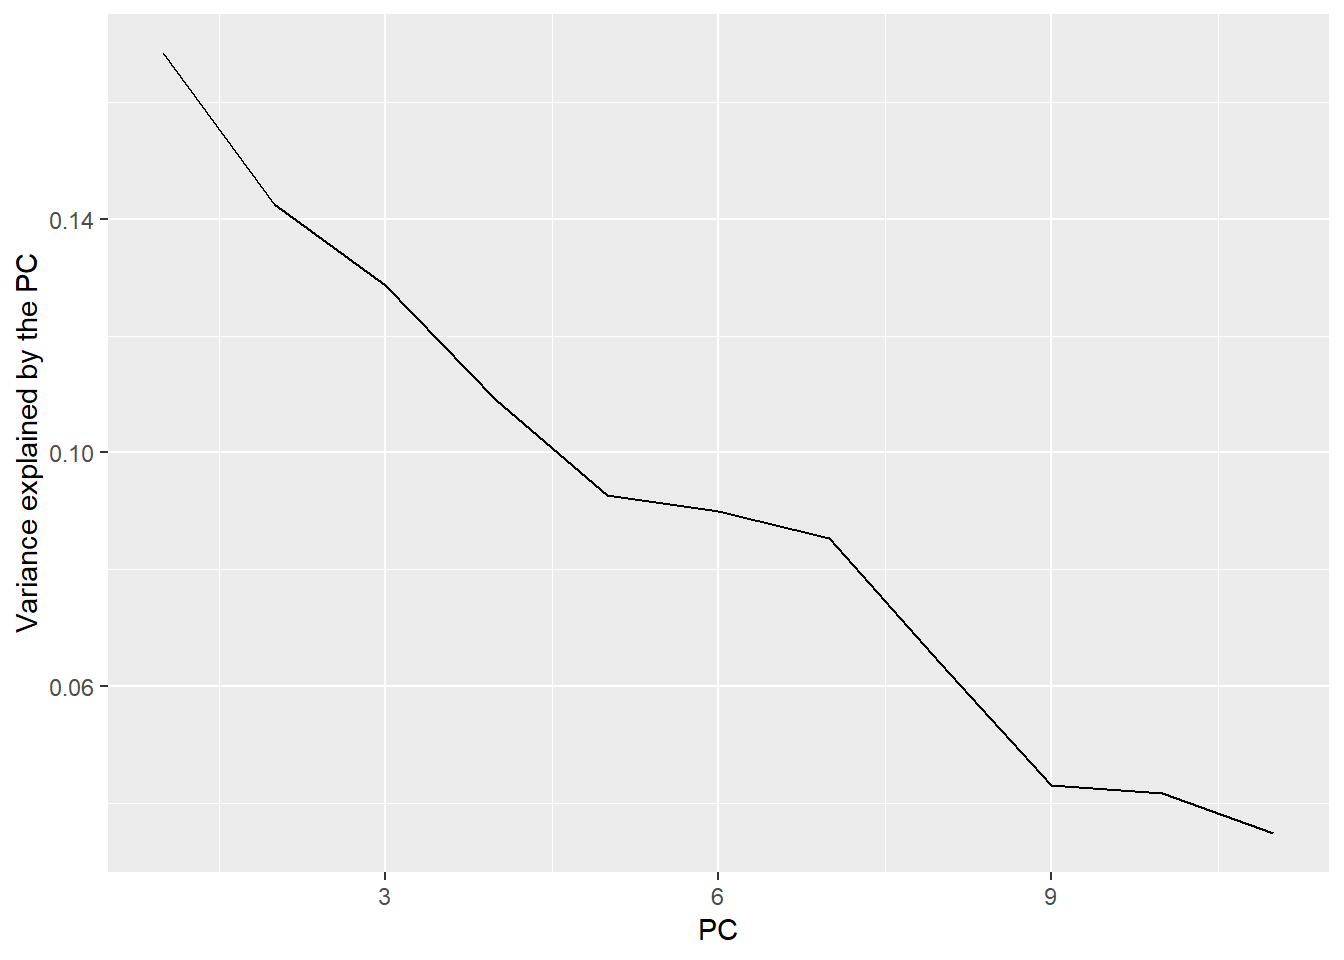
\includegraphics[width=0.8\linewidth]{CVEN6833-Project_files/figure-latex/lambdas-1} 

}

\caption{Variance explained by each PC}\label{fig:lambdas}
\end{figure}

\begin{figure}

{\centering 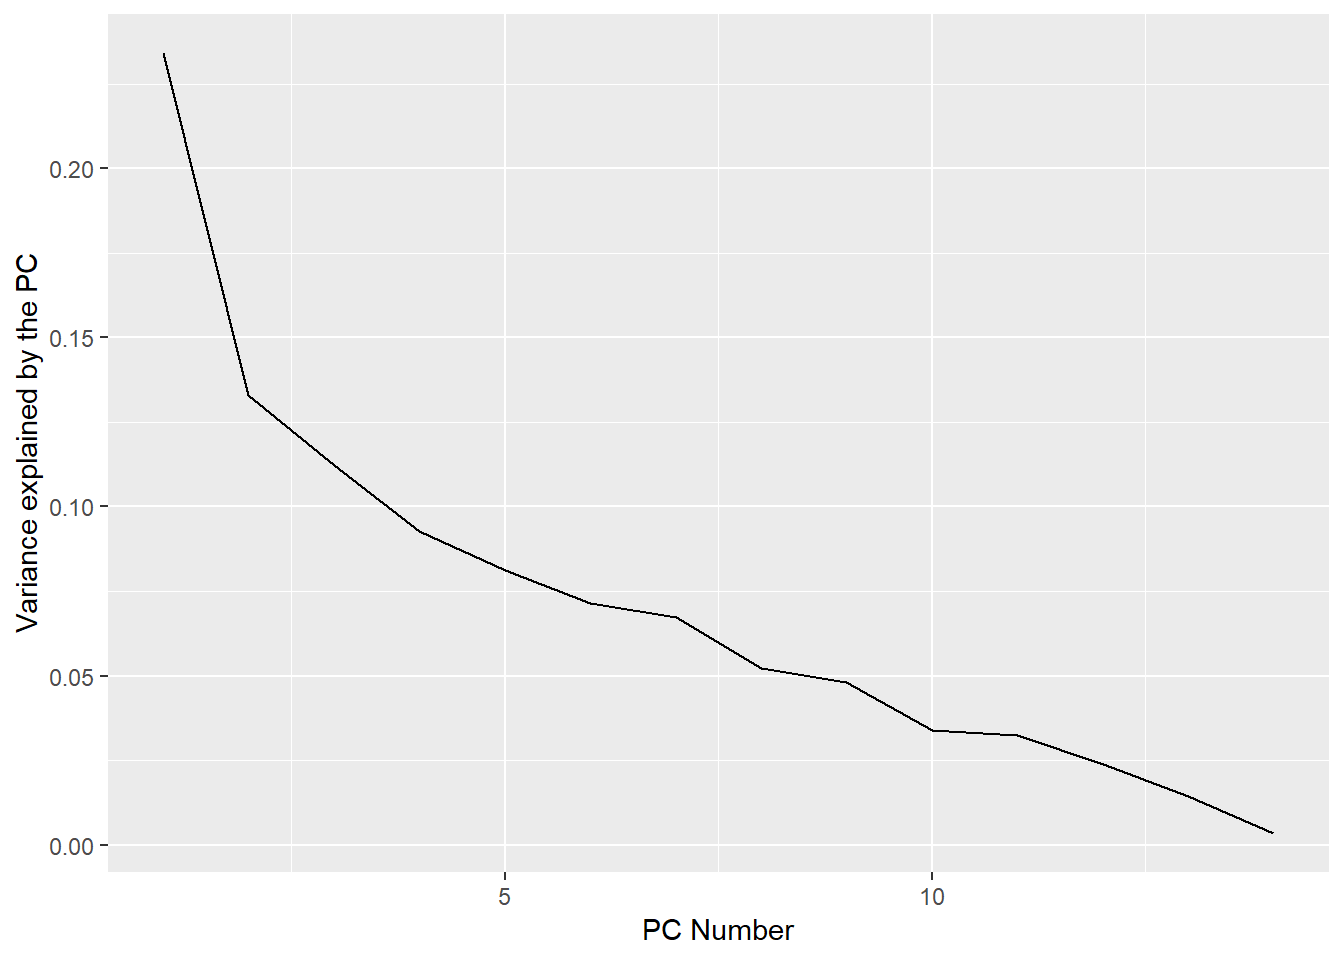
\includegraphics[width=0.8\linewidth]{CVEN6833-Project_files/figure-latex/lambdas-clim-1} 

}

\caption{Variance explained by each PC, including climate variables}\label{fig:lambdas-clim}
\end{figure}

With the second analysis (climate - considered), the influence of each
eigenvector on the attributes of our dataset was plotted and analyzed
(fig. \ref{fig:eigen})

\begin{figure}

{\centering 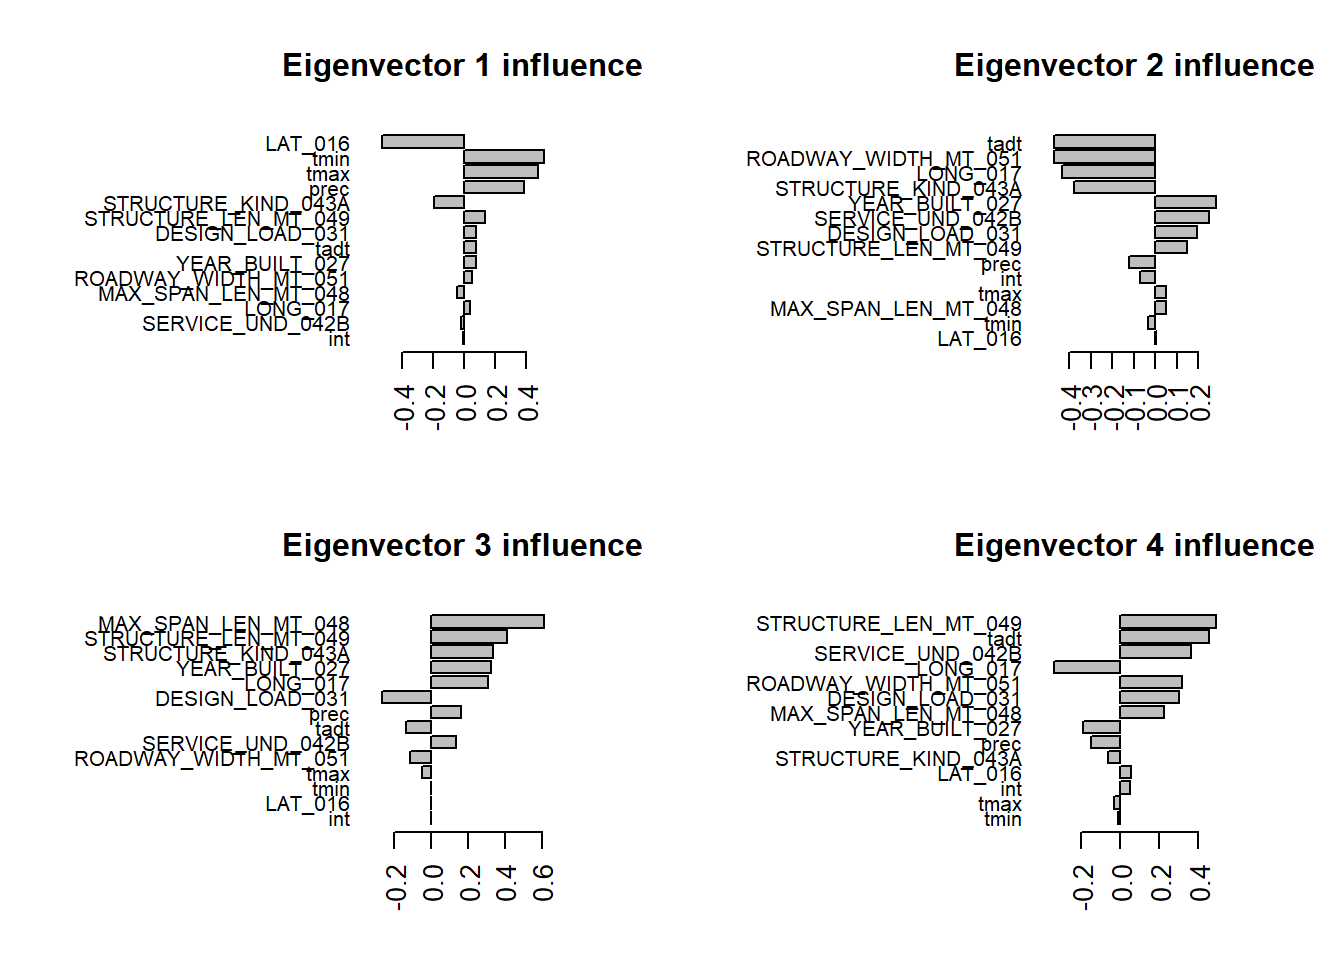
\includegraphics[width=1\linewidth]{CVEN6833-Project_files/figure-latex/eigen-1} 

}

\caption{Influence of eigenvector on each attribute}\label{fig:eigen}
\end{figure}

\subsection{Multinomial regression}\label{multinomial-regression}

The first 4 PC were used to fit a multinomial regression on the
structural condition of the bridge, as they represent almost 60\% of the
variance of the model. The best model using step AIC criteria was the
one including all four PC as covariates.

Two statistics were calculated to assess the accuracy of the regression.
First, the ranked probability score for the model without climate
variables was of 7.5 \%. That is, the increase in the accuracy by
predicting through the model instead of the count based probabilities
was of 7.5 \%. The introduction of the climate variables (tmax, tmin,
prec) increased the ranked probability score skill from 7.5 \% to 8.6
\%.

Additionally, a confusion matrix \texttt{caret::confusionMatrix} was
calculated to evaluate the ``false positives'' and ``false negatives''
the model predicted. The output shown below evidences how hard it is for
the model to be accurate, as the number of ``false 1 identified as
such'' (structurally deficient) is similar to non identified ``true 1''.
Only a small fraction of ``true 1'' are identified correctly.

\begin{verbatim}
##           Reference
## Prediction    1    2    3
##          1   78  151  613
##          2  144  303 1249
##          3  633 1236 8563
\end{verbatim}

\section{Self Organizing Maps}\label{self-organizing-maps}

As an alternative to the previous machine learning techniques, a 3 by 3
node SOM clustering has been carried out. Figure \ref{fig:som-plot} the
weight of each attribute on each of the 9 nodes. The resulting
distribution aggregates statistically closer bridges in the same nodes,
with a potential for better accuracy in the regression of each
separately.

\begin{figure}

{\centering 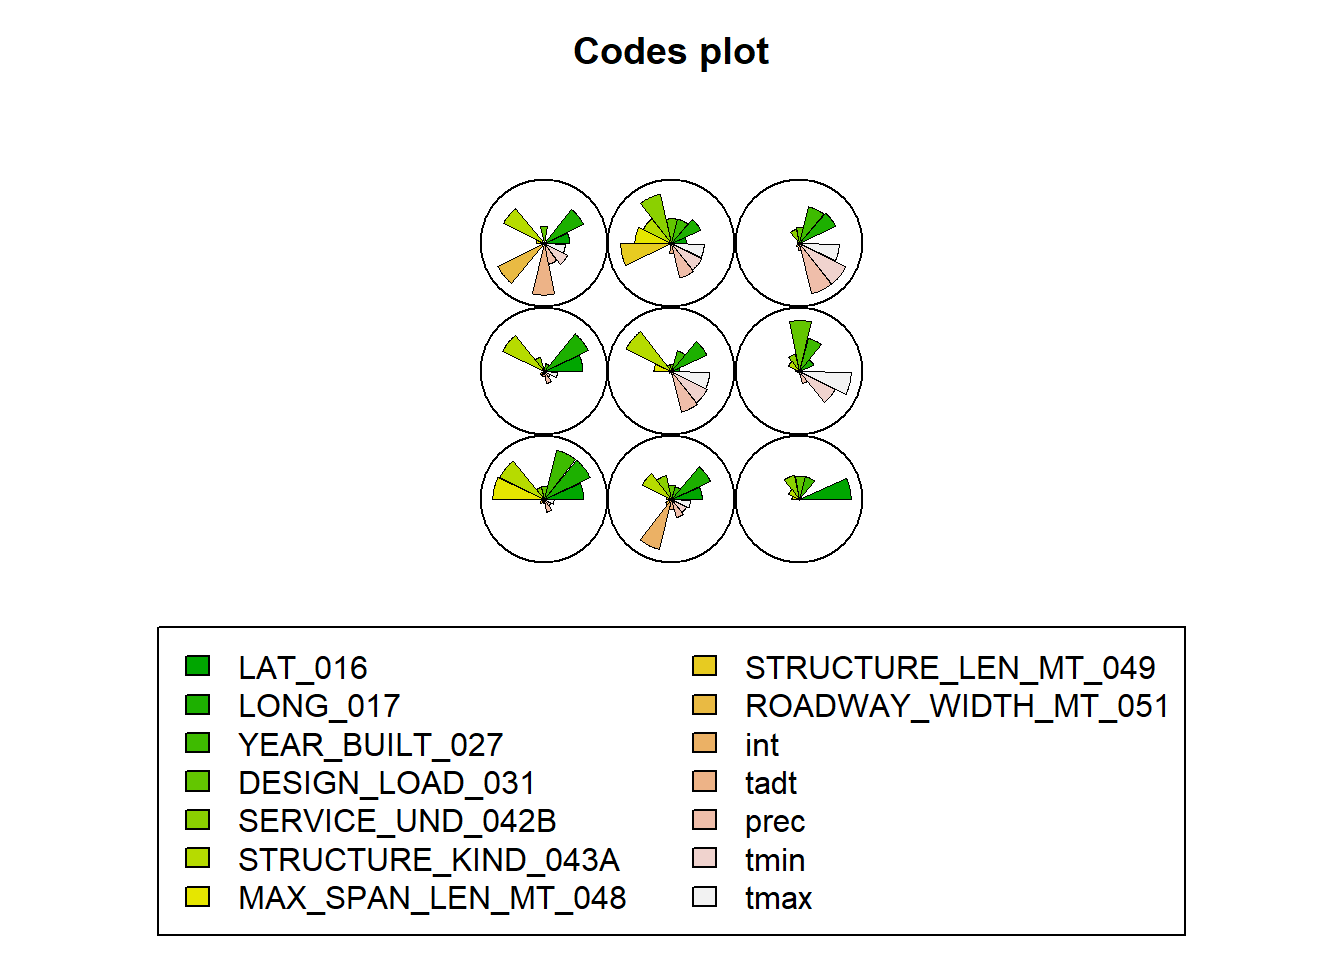
\includegraphics[width=1\linewidth]{CVEN6833-Project_files/figure-latex/som-plot-1} 

}

\caption{Attribute (code) signal on each node}\label{fig:som-plot}
\end{figure}

To better explain this approach, two properties from the ensemble, the
design load knowledge and the reconstruction effect, will be plotted.
Figure \ref{fig:som-prop1} shows the strong signal of the design load
variable on the red node. Similarly, the comparative relevance of
bridges on an specific node related to the binary variable
``reconstruction'' is plotted in figure \ref{fig:som-prop2}.

\begin{figure}

{\centering 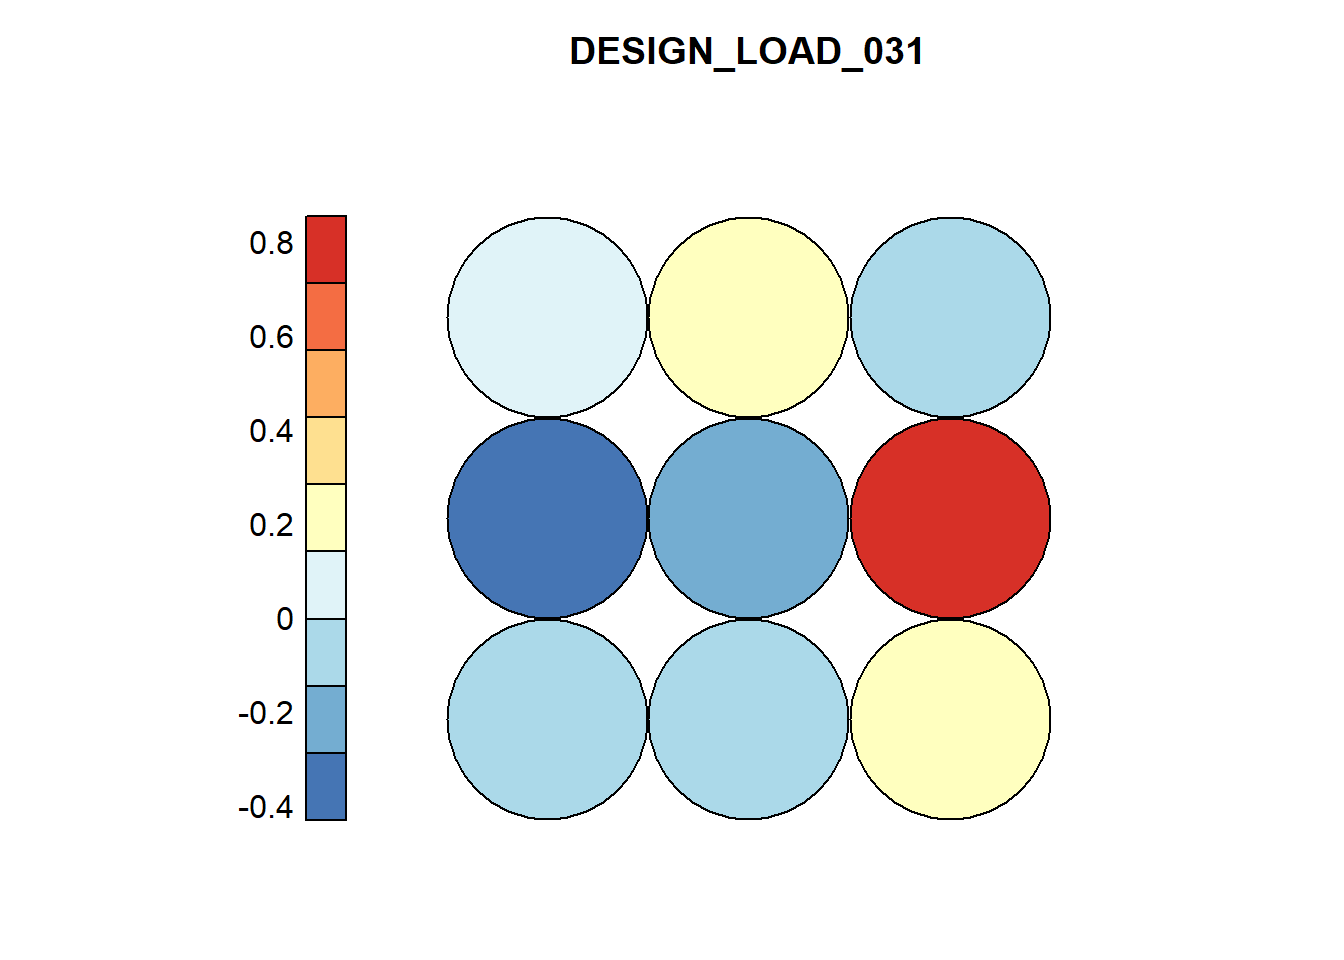
\includegraphics[width=0.8\linewidth]{CVEN6833-Project_files/figure-latex/som-prop1-1} 

}

\caption{Property plot for "Design load" binary variable}\label{fig:som-prop1}
\end{figure}\begin{figure}

{\centering 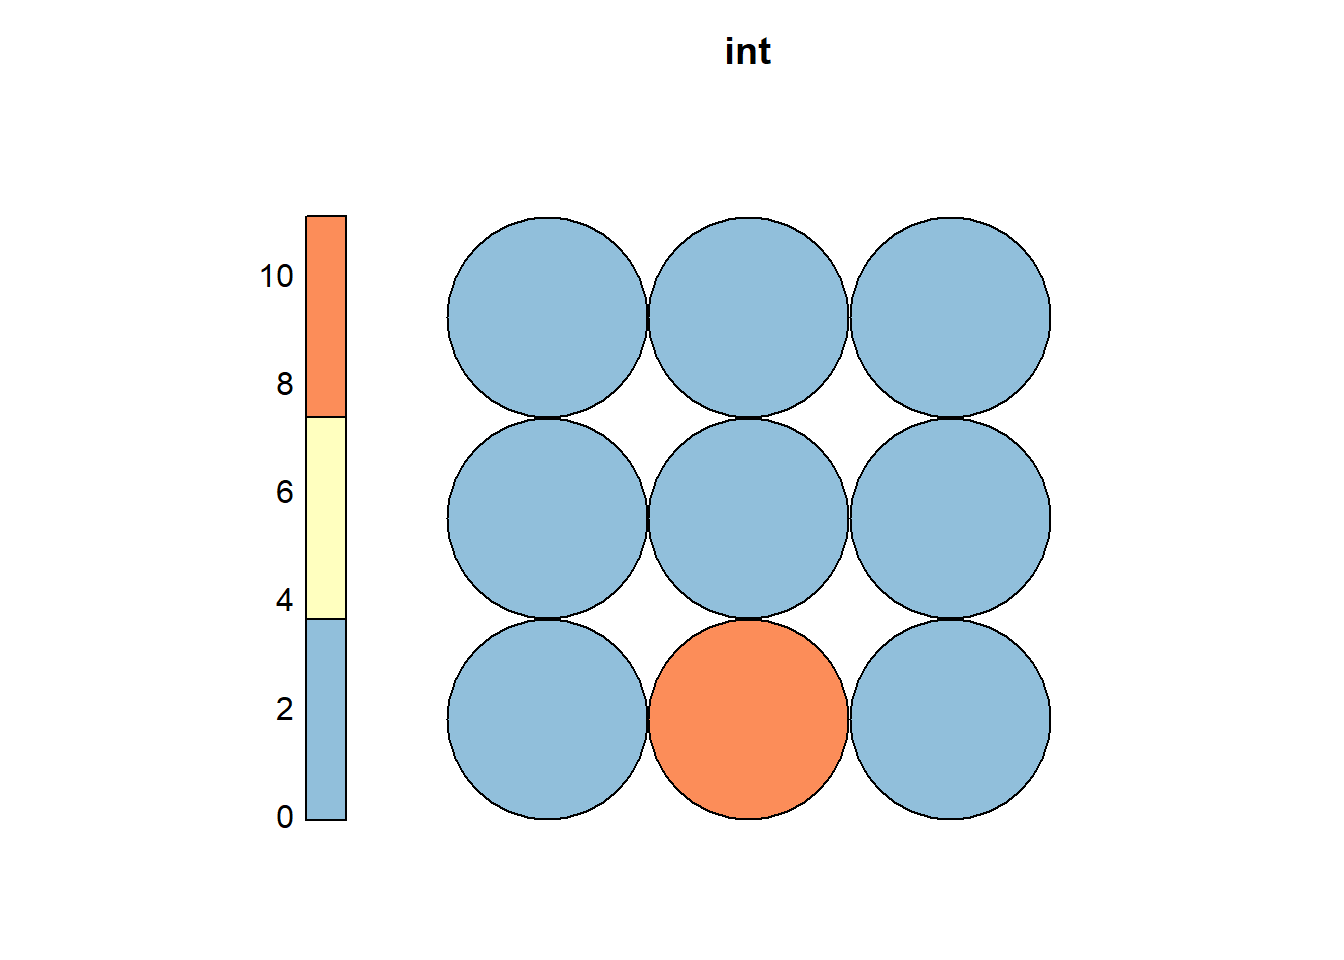
\includegraphics[width=0.8\linewidth]{CVEN6833-Project_files/figure-latex/som-prop2-1} 

}

\caption{Property plot for "Reconstruction" binary variable}\label{fig:som-prop2}
\end{figure}

Alternatively, a hierarchical clustering could be carried out on the map
to obtain fewer number of nodes and reduce regression models. As an
example, a k-means with 4 clusters on the nodes is showed in figure
\ref{fig:som-cluster}.

\begin{figure}

{\centering 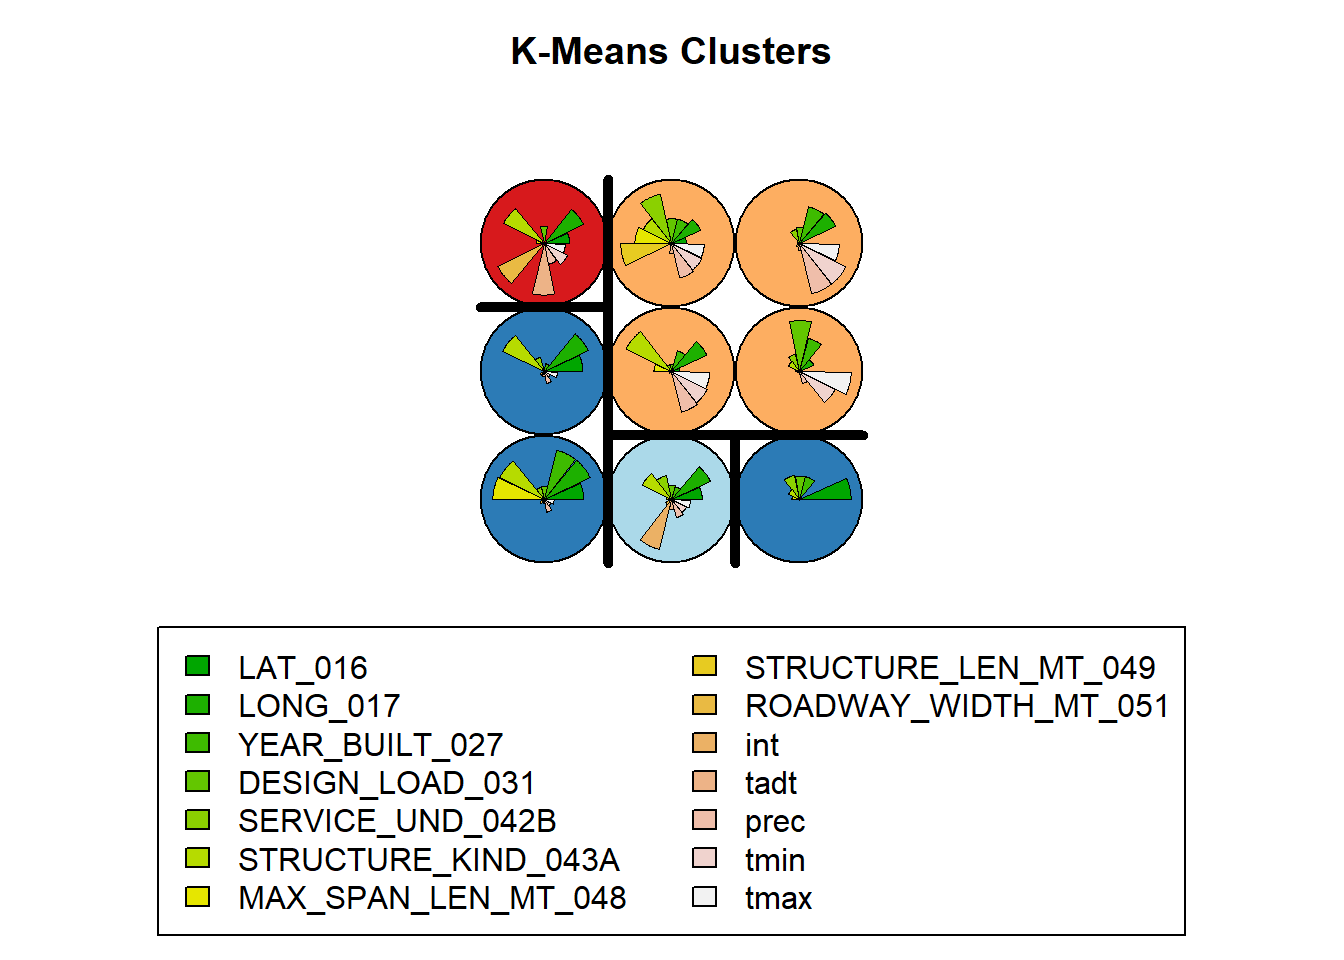
\includegraphics[width=1\linewidth]{CVEN6833-Project_files/figure-latex/som-cluster-1} 

}

\caption{Hierarchical K-means clustering on SOM}\label{fig:som-cluster}
\end{figure}

\bibliography{references.bib,packages.bib}


\end{document}
